% -*-LaTeX-*-

\section{Implementation}
\label{sec:impl}

%
% Outline of the implementation
%    - back storage
%    - libpfs
%    - pfsd + FUSE
% Why we implemented pFS as a library
%   easy to use API for working with our versionning system
%   independant of the communication layer used to propagate updates
% Layout of the back storage
%   ~/.pfs/data
%   ~/.pfs/info
%   ~/.pfs/groups
%   groups information (participating sd) contained in pFS itself
%   so that it gets propagated
% libpfs
%    layout of the exposed file system
%    pfs_instance -> link to back storage
%                    opened files
%    POSIX API
%       what happens :
%       path lookup -> need for caching
%       when file modified link (old_id, new_id) + update vv +
%                        pfs_set_entry
%            relinking + file close -> happen on back storage
%            update vv + pfs_set_entry happen in memory
%       pfs_sync_cache
%    updt as argument of set_entry
%    pfs_set_updt_cb
%    pfs_apply_updt
%    => layer above libpfs has access to POSIX I/F, receive updt
%        struct as callbacks for propagation and must apply locally
%        the updts it receive + putting the ressource in data/
% pfsd
%    couple of line FUSE stub
%    in charge of update propagation : need for a log
%    our prototype using IP
%       Need for a naming service (DNS ?)
%       Need for relay servers (Devices being firewall)
%       transmitting updates : simple transmission of pfs_updt struct
%       transmitting data : simple data transmission, LBFS/rsync
%                           should be used
%    prototype using Bluetooth
%       no naming service / relay : service exported and devices
%       attached
%   LAN transmission priority
%   Future work : need for transmission layer decision


We implemented pFS as a two level architecture based on the device
local file system :

\begin {itemize}
\item \textbf{Back storage} : a directory on the local file system
  containing all data and metadata used and generated by pFS.
\item \textbf{libpfs} : the core functionalities of pFS related to
  versionning are implemented in libpfs which exports a POSIX file
  system interface along with extra functionalities specific to
  pFS.
\item \textbf{Fuse stub} : exports pFS to the user as a file
  system. It translates directly the calls received from
  Fuse~\cite{henk:fuse} to the POSIX file system interface exported by
  libpfs.
\item \textbf{pfsd} : a daemon that is responsible for propagating
  updates using any communication channel available and apply updates
  received from other devices. pfsd receives callbacks from libpfs
  whenever an update is made locally, and use libpfs API to commit
  updates received from remote devices on the local device.
\end {itemize}

\begin{figure}[ht]
\begin{center}
  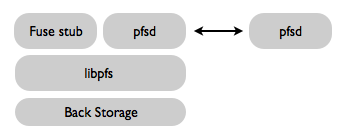
\includegraphics [scale=0.6] {img/impl}
  \caption{\label{PfsImpl} {\small pFS Implementation as a two level
      architecture based on the device local file system}}
\end{center}
\end{figure}

We designed the core component of pFS as a library in order to provide
an easy-to-use API for taking advantage of our versionning system that
is independent of the communication channels used to propagates the
updates between the different $sd$s.

\subsection {Back Storage}

The back storage is layed out as follows : \\ {\tt /.pfs/data/}
\\ {\tt /.pfs/dir/} \\ {\tt /.pfs/info} \\ {\tt /.pfs/groups} \\

{\tt /.pfs/info} is a file containing the user unique id, the storage
device unique id, along with the user name and the device name. {\tt
  /.pfs/groups} contains the list of the groups the device is involved
in, with for each group the unique id of the {\tt pfs\_dir} structure
representing the root of the group tree. {\tt /.pfs/dir/} contains one
file per {\tt pfs\_dir} structure existing in the system, named after the {\tt
  pfs\_dir} unique id. It contains a serialized version of the {\tt
  struct pfs\_dir} used by the versionning system and described in
Figure \ref{MemStruct}. As we described in section \ref{sec:vers}
entries in {\tt pfs\_dir} are versionned and each version contains
a type and an unique id. If the type of the version is
$DIR$, the id refers to a file in {\tt /.pfs/dir/}, otherwise, if the
type of the version is $FIL$, the id refers to a file in {\tt
  /.pfs/data/} containing the actual content of the file. The list of
$sd$s participating in a group is contained in pFS itself such that it
gets propagated and can be handled directly by pfsd.

\subsection {libpfs}

The pFS file system exposed to the user through Fuse is layed out as
follows : the root directory contains a list of directories
representing each group in which the device is involved. The initial
group on any device is {\tt me} and involves all the devices that
belongs to the owner of that device.

Since libpfs is structured as a library, all functions get a {\tt
  pfs\_instance} structure as argument. This structure contains the path
of the back storage and the list of currently opened files. libpfs
exports a POSIX-like file system API : {\tt pfs\_open}, {\tt
  pfs\_close}, {\tt pfs\_pwrite}, {\tt pfs\_unlink}... These calls get
absolute paths (containing the group directory) as argument for file
or directory operations mainly in order to be compliant with Fuse API
which uses absolute paths from the root of the mounted file system.

Therefore, we need to walk down the chain of {\tt pfs\_dir} structures
anytime an operation has to be made on a file that has no associated
file handler. Since {\tt pfs\_dir} structures are stored in files
contained in {\tt /.pfs/dir/} we have implemented a cache in order to
walk theses structures in memory and avoid having to open and read as
many file as the depth of the path we are given as argument. The cache
is a simple LRU cache implemented with a hash table mapping {\tt
  pfs\_dir} id to the actual in-memory data structure. It does not
need to be large since modifications made inside a directory results in
many requests to the same {\tt pfs\_dir} structures. In our
implementation we are caching 64 {\tt pfs\_dir} structures, a pointer
to the cache is stored in the {\tt pfs\_instance} structure. libpfs
provides a {\tt pfs\_sync\_cache} function for periodically writing
back the cache to disk (every 10s in our implementation of pfsd). The
cache has incurred an important improvement over the performances of
libpfs since {\tt pfs\_dir} fetchs and write backs are amortized over
a lot of operations in case of intensive workloads, or appear as
asynchronous for less intensive workloads.

\paragraph{Local file operations :}
When a file is created, a new unique id is generated, the associated
file is created in {\tt /.pfs/data/} and a {\tt pfs\_set\_entry} call
is issued to insert the new {\tt pfs\_ver} into the {\tt pfs\_dir}
associated with the directory in which the file is created. The file
creation happens on the back storage file system while the version
update happens in memory using the cache we described. Opening a file
for reading does not need to update any versioning information and is
directly mapped to an {\tt open} call on the back storage file. Therefore
creating a file or opening a file for reading using pfslib incurs
almost no overhead. 

At the contrary, opening a file for writing necessitates the
generation of a new unique id. This new mapping is needed as soon as
the {\tt pfs\_open} call is issued since the actual id for the file
might be revoked if an update containing a dominating version is
received while the file is edited. The {\tt pfs\_ver} associated with
the newly generated id is inserted in memory when the file is
subsequently closed. Therefore opening a file for writing using libpfs
incurs a non negligeable overhead and maps to two calls on the back
storage : {\tt link (old\_id, new\_id)} and {\tt open (new\_id)}.

Merging a version into the local main version is translated into a
call to {\tt pfs\_set\_entry}, and an {\tt unlink} call to the back
storage to revoke the version that has been superseded.

\paragraph{Local directory operations :}
Directory creation are mapped to the creation of a file in {\tt
  /.pfs/dir/}, the insertion of a {\tt pfs\_dir} structure in the
cache and the update of the parent {\tt pfs\_dir} (already present in
the cache). Directory removals are mapped to an {\tt unlink} call to
the back storage, the removal of an entry in the cache and the update
of the parent {\tt pfs\_dir}. Therefore, directory operations using
libpfs incurs a slight overhead by mapping directory operations to
back storage files operations and in memory updates.

\paragraph{}

libpfs also provides interfaces used for two-way communication of
updates with pfsd. Functions can be registered to be called
any time a {\tt pfs\_set\_entry} is issued. The argument passed to
those callbacks is a {\tt pfs\_updt} structure that contains all the
arguments needed to issue the same {\tt pfs\_set\_entry} on another
device :

\begin{figure}[ht]
\begin{center}
{\tt \small
\begin{verbatim}
struct pfs_updt
{
  char grp_id [PFS_ID_LEN];
  char dir_id [PFS_ID_LEN];  
  char name [PFS_NAME_LEN];
  uint8_t reclaim;
  struct pfs_ver * ver;
};
\end{verbatim}
}
\end{center}
\caption{\label{MemStruct}
{\small {\tt pfs\_updt} structure propagated by pfsd among the
    different instances of libpfs.}}
\end{figure}

The updates received by pfsd from the network can be applied to the
local copy of pFS by calling {\tt pfs\_set\_entry} directly.

\subsection {pfsd}

We have implemented a simple version of pfsd using IP as a transport
layer. We used a very simple protocol allowing to send updates from
one device to another and retransmit associated files contained in {\tt
  /.pfs/data}. In the context of IP, a naming service is needed to
enable the devices to discover each others' address from
their unique ids. DNS can be used as such naming service. In our
prototype, we designed a simple centralized naming service to which
devices would register when they were connected. Such naming service
is not always needed. As an example, a daemon using Bluetooth
would rely on the built-in mechanisms to attach devices such that they
recognize each others when placed at proximity.

There is no final design for pfsd since it is highly dependent on which
type of device and which type communication channel it relies on. This
section is rather a survey of lessons and directives we have learnt
from designing our prototype of pfsd. 

\paragraph {The role of pfsd :}
\begin{itemize}
\item propagate to other devices the updates generated locally.
\item receive update from other devices and apply them to the local
  instance of libpfs.
\end{itemize}

\paragraph {Update Logging :}
pfsd need to maintain a log of every update it sees in order to
retransmit them to other devices. Two important points have to be
considered when implementing update logging :
\begin{itemize}
\item The callbacks used by libpfs to transmit local updates to pfsd are
  placed on the critical execution path of any local
  operation. Therefore, when received, updates should be temporarely
  stored in memory before being writtem back asyncrhonously to permanent
  storage.
\item Depending on the context, updates should be augmented by pfsd
  with a propagation vector to keep track of which devices have
  already receive any given update.
\item Any update that has been propagated to all devices can and
  should be removed from the log to avoid wasting local storage
  capacity.
\end{itemize}

\paragraph {File transmission :}
Along with the updates, back storage files stored in {\tt /.pfs/data/}
have to be transmitted between the devices. Back storage files
associated with different version of a same file are very likely to be
similar. rsync\cite{tridgell:rsync} as well as concepts introduced in
LBFS\cite{muthitacharoen:lbfs} should definitely be considered for
file transmission in order to avoid wasting bandwidth.

\paragraph {Choice of communication channel:}
If different communication channels are available (IP (LAN / WAN),
Bluetooth, Wire), it is essential to define a policy to decide which
layer to use given the updates to be propagated. It would be
inefficient to propagate GB of data over WAN from a desktop computer
at home to a desktop computer at work if this data can be quickly
pushed to a mobile device such as a cell phone that will be able to
rapidly deliver the data when it will be at proximity of the desktop
computer at work. Please refer to section \ref{sec:futwk} for a more
extensive discussion of this issue.

% Local Variables:
% tex-main-file: "main.ltx"
% tex-command: "make;:"
% tex-dvi-view-command: "make preview;:"
% End:
